\chapter{Graph-Based SLAM  Grisetti}
{\large A Tutorial on Graph-Based SLAM}

\section{Abstract}
Provide an introductory description to the graph-based SLAM problem. Furthermore, we discuss a state-of-the-art solution that is based on least-squares error minimization and exploits the structure of the SLAM problems during optimization. The goal of this tutorial is to enable the reader to implement the proposed methods from scratch. 

\section{Preamble}
\textbf{SLAM}: Simultaneous Localization and Mapping -- Learning maps under pose uncertainty.

\textbf{Motivation for SLAM}: To efficiently solve many tasks envisioned to be carried out by mobile robots including transportation, search and rescue, or automated vacuum cleaning robots need a map of the environment. The availability of an accurate map allows for the design of systems that can operate in complex environments only based on their on-board sensors and without relying on external reference system like, e.g., GPS.

\textbf{Brief taxonomy for SLAM solutions}:
\begin{enumerate}
    \item \textbf{filtering}: Filtering approaches model the problem as an on-line state estimation where the state of the system consists in the current robot position and the map. The estimate is augmented and refined by incorporating the new measurements as they become available. To highlight their incremental nature, the filtering approaches are usually referred to as on-line SLAM methods.
    \begin{itemize}
        \item Kalman filter and Extended Kalman filter.
        \item Information filter and Extended information filter.
        \item Particle filter.
    \end{itemize}
    \item \textbf{smoothing}: smoothing approaches estimate the full trajectory of the robot from the full set of measurements. These approaches address the so-called full SLAM problem, and they typically rely on least-square error minimization techniques.
\end{enumerate}

\textbf{What can SLAM do}: 
% \begin{figure}[htbp]
%     \centering
%     \begin{minipage}[t]{0.3\textwidth}
%         \centering
%         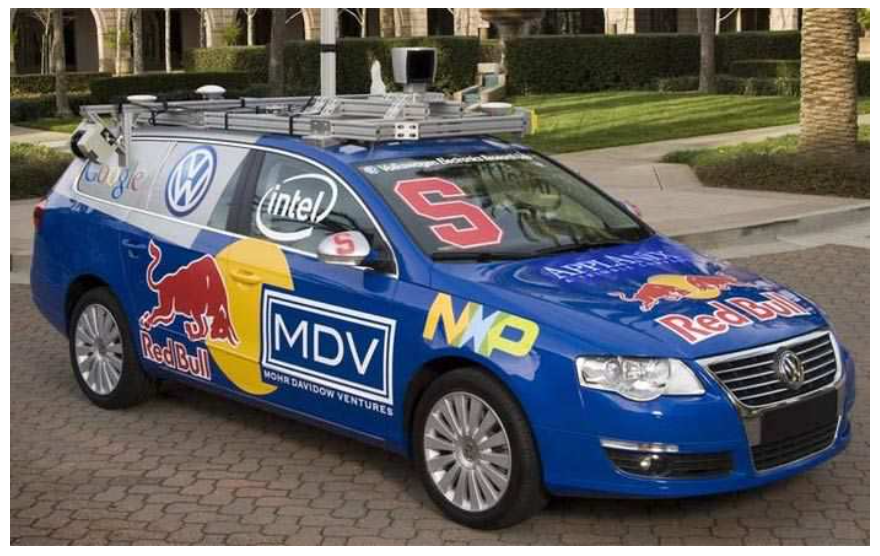
\includegraphics[scale=0.3]{figures/graph_slam/autonomous_parking.png}
%         \caption{Autonomous parking in parking garage}
%     \end{minipage}
%     \begin{minipage}[t]{0.3\textwidth}
%         \centering
%         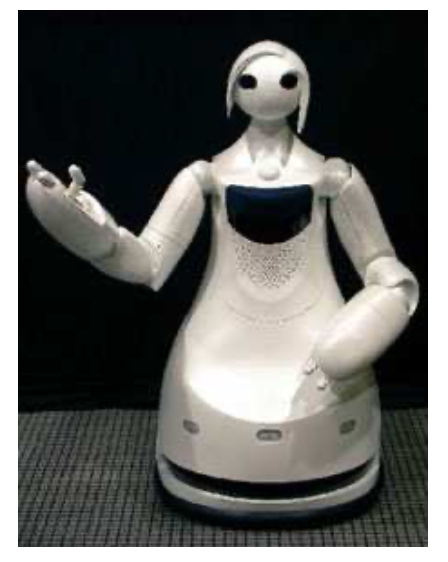
\includegraphics[scale=0.3]{figures/graph_slam/tour_guide.png}
%         \caption{Guiding tours in museum}
%     \end{minipage}
%     \begin{minipage}[t]{0.3\textwidth}
%         \centering
%         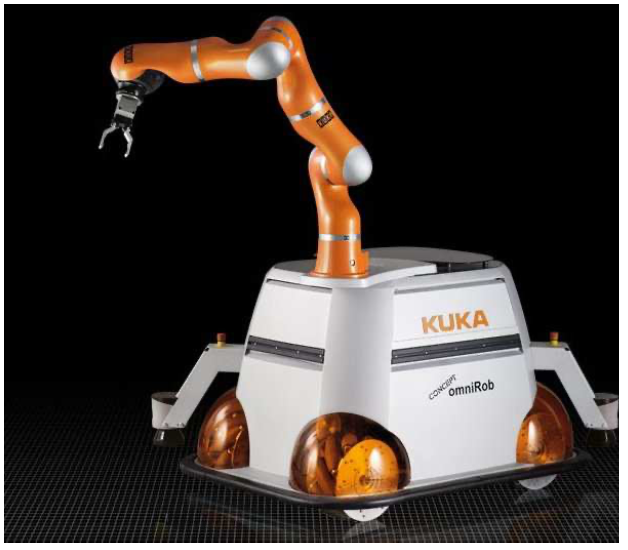
\includegraphics[scale=0.3]{figures/graph_slam/flexible_induestrial_manipulator.png}
%         \caption{Flexibly navigating and operating in changing industrial environment}
%     \end{minipage}
%     % \caption{}
%     \label{fig:what_can_slam_do}
% \end{figure}
\begin{figure}[htbp] 
    \centering
    \subcaptionbox{Autonomous parking in parking garage}{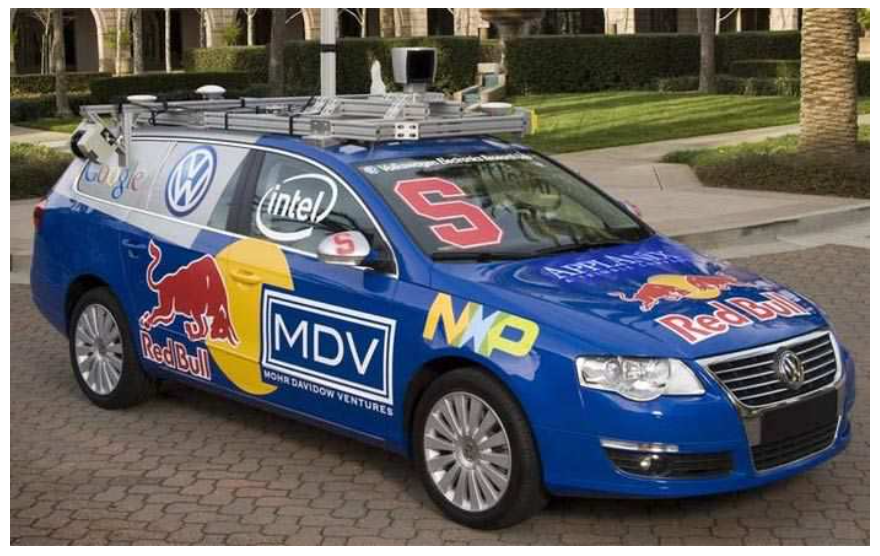
\includegraphics[width=0.3\textwidth]{figures/graph_slam/autonomous_parking.png}}
    \hfill
    \subcaptionbox{Guiding tours in museum}{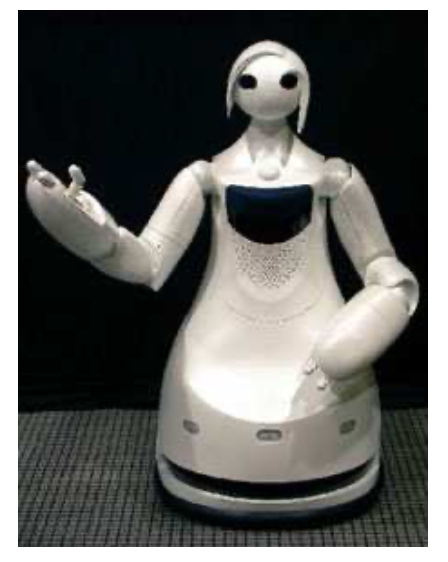
\includegraphics[width=0.3\textwidth]{figures/graph_slam/tour_guide.png}}
    \hfill
    \subcaptionbox{Flexibly navigating and operating in changing industrial environment}{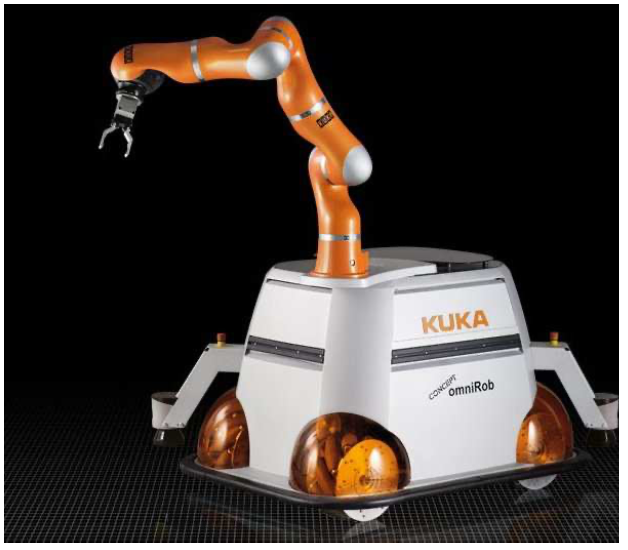
\includegraphics[width=0.3\textwidth]{figures/graph_slam/flexible_induestrial_manipulator.png}}
    \caption{What SLAM can do}
    \label{fig:what_slam_can_do}
\end{figure}

\textbf{Grisetti's elaboration for Graph-Based SLAM}: Solving a graph-based SLAM problem involves to construct a graph whose nodes represent robot poses or landmarks and in which an edge between two nodes encodes a sensor measurement that constrains the connected poses. Obviously, such constraints can be contradictory since observations are always affected by noise. Once such a graph is constructed, the crucial problem is to find a configuration of the nodes that is maximally consistent with the measurements. This involves solving a large error minimization problem. 

\textbf{Grisetti's elaboration for evolution of Graph-Based SLAM}: The graph-based formulation of the SLAM problem has been proposed by Lu and Milios in 1997. However, it took several years to make this formulation popular due to the comparably high complexity of solving the error minimization problem using standard techniques. Recent insights into the structure of the SLAM problem and advancements in the fields of sparse linear algebra resulted in efficient approaches to the optimization problem at hand. Consequently, graph-based SLAM methods have undergone a renaissance and currently belong to the state-of-the-art techniques with respect to speed and accuracy.

\section{Probabilistic formulation of full SLAM}
\textbf{Why probabilistic}: Due to the inherent noise in the sensor measurements. 

\textbf{Full SLAM problem}: 
\begin{equation}
    p(x_{1:t}, m | x_0, u_{1:t}, z_{1:t})
    \label{equ:full_slam_prob}
\end{equation}

\textbf{A bif of elaboration}: 
\begin{enumerate}
    \item The initial position $x_0$ defines the position of the map and can be chosen arbitrarily. Therefore, $x_0$ is always omitted in some SLAM formulations.
    \item The poses and the odometry are usually represented as 2D or 3D transformations in $SE(2)$ or in $SE(3)$.
    \item The map can be represented in different ways ({\color{red} \emph{Need more specific taxonomy of representations of map in SLAM}}):

    \begin{figure}[htbp]
        \centering
        \subcaptionbox{Multilevel surface maps}{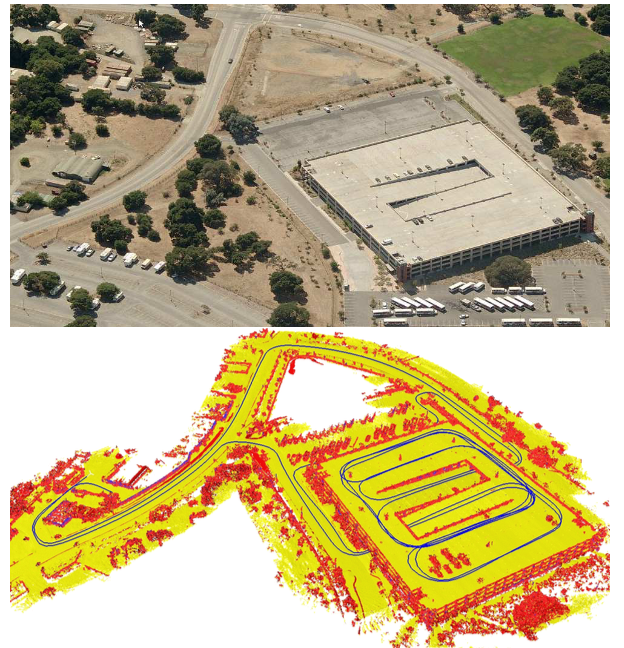
\includegraphics[width=0.3\textwidth]{figures/graph_slam/multilevel_surface_map.png}}
        \hfill
        \subcaptionbox{Point clouds map}{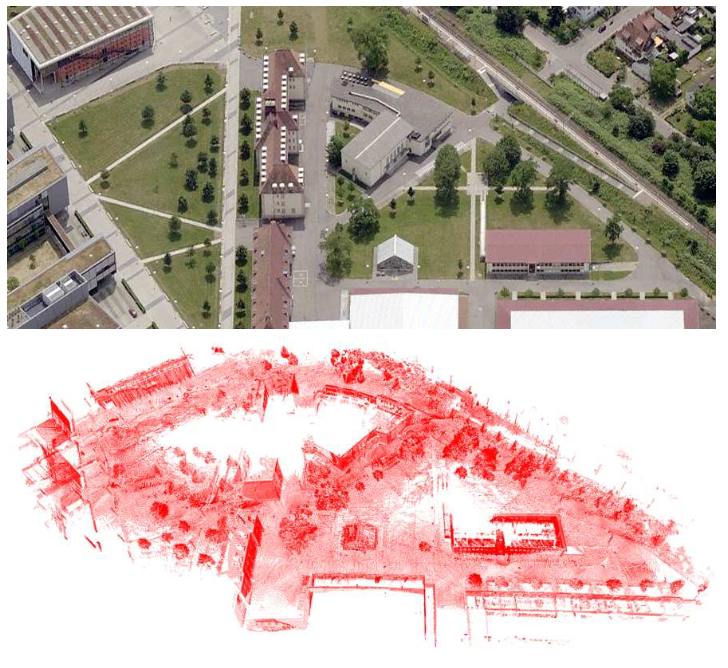
\includegraphics[width=0.3\textwidth]{figures/graph_slam/point_clouds_map.png}}
        \hfill
        \subcaptionbox{Occupancy grid map}{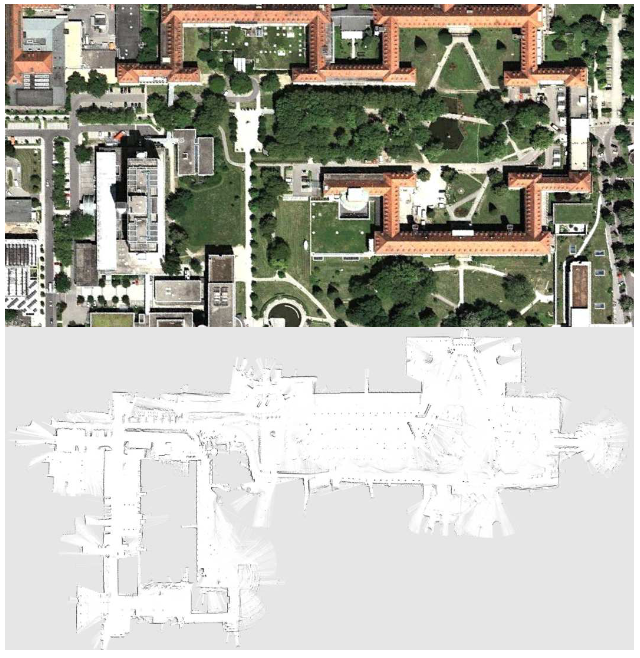
\includegraphics[width=0.3\textwidth]{figures/graph_slam/occupancy_grid_map.png}}
        \caption{Dense representations of the map}
        \label{fig:map_dense_representations}
    \end{figure}
    \begin{itemize}
        \item Maps can be parametrized as a set of spatially located landmarks, by dense representations:
        \begin{itemize}
            \item occupancy grids.
            \item point clouds.
            \item multilevel surface maps.
        \end{itemize}
        \item Or by raw sensor measurements.
    \end{itemize}
    \item The choice of a particular map representation depends on the sensors used, on the characteristics of the environment, and on the estimation algorithm. 
    \item Landmark maps are often preferred in environments where locally distinguishable features can be identified and especially when cameras are used. In contrast, dense representations are usually used in conjunction with range sensors. Independently of the type of the representation, the map is defined by the measurements and the locations where these measurements have been acquired.
\end{enumerate}

\section{Graphical formulation of full SLAM}
\textbf{Motivation for using graphical model}: Estimating the posterior given in \ref{equ:full_slam_prob} involves operating in high dimensional state spaces. This would not be tractable if the SLAM problem would not have a well defined structure. 

\begin{figure}[htbp]
    \centering
    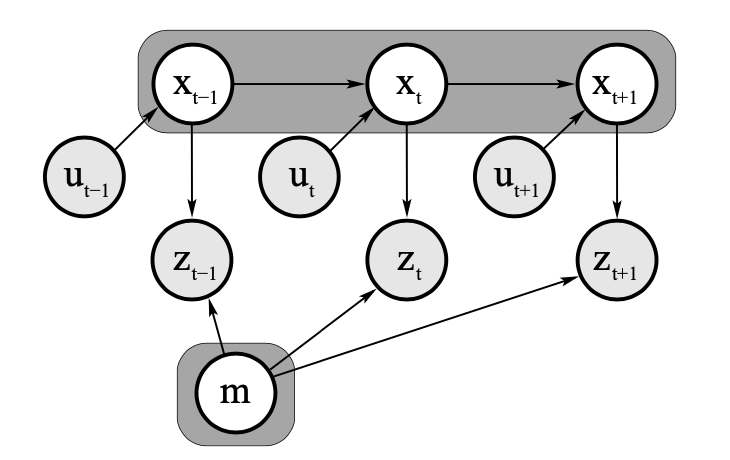
\includegraphics[width=0.5\textwidth]{figures/graph_slam/full_slam_graphical_model.png}
    \caption{Dynamic Bayesian Network of the full SLAM process}
    \label{fig:full_slam_dbn}
\end{figure}


\textbf{Dynamic Bayesian Network}: A convenient way to describe this structure is via the Dynamic Bayesian Network (DBN) depicted in Figure~\ref{fig:full_slam_dbn}. A Bayesian network is a graphical model that describes a stochastic process as a directed graph. The graph has one node for each random variable in the process, and a directed edge between two nodes models a conditional dependence between them. In Figure~\ref{fig:full_slam_dbn}, one can distinguish blue/gray nodes indicating the observed variables and white nodes which are the hidden variables. The hidden variables $x_{1:t}$ and $m$ model the robot’s trajectory and the map of the environment. The connectivity of the DBN follows a recurrent pattern~\footnote{A \textbf{Recurrent Neural Network (RNN)} basically unfolds over time. It is used for sequential inputs where the time factor is the main differentiating factor between the elements of the sequence. A \textbf{Recursive Neural Network} is more like a hierarchical network where there is really no time aspect to the input sequence but the input has to be processed hierarchically in a tree fashion.} characterized by the state transition model and by the observation model. 

\section{Graph-Based formulation of full SLAM}
In contrast to DBN which highlights the \emph{temporal}\footnote{This temporal structure makes this formalism well suited to describe filtering processes} structure of the full SLAM problem, the graph-based formulation highlights the underlying \emph{spatial} structure.

\textbf{Basic idea}: A graph-based SLAM algorithm constructs a graph out of the raw sensor measurements. Each node in the graph represents a robot position and a measurement acquired at that position. An edge between two nodes represents a spatial constraint relating the two robot poses. A constraint consists in a probability distribution over the relative transformations between the two poses. These transformations are either odometry measurements between sequential robot positions or are determined by aligning the observations acquired at the two robot locations. Once the graph is constructed one seeks to find the configuration of the robot poses that best satisfies the constraints.

\textbf{Two tasks}: 
\begin{enumerate}
    \item \textbf{Graph construction}: constructing the graph from the raw measurements. The graph construction is usually called \emph{front-end} and it is heavily sensor dependent.
    \item \textbf{Graph optimization}: determining the most likely configuration of the poses given the edges of the graph. The graph optimization is called \emph{back-end} and relies on an abstract representation of the data which is sensor agnostic.
\end{enumerate}

\textbf{More elaboration about front-ends and back-ends}: Most optimization techniques focus on computing the best map given the constraints and are called SLAM \emph{back-ends}. In contrast to that, SLAM \emph{front-ends} seek to interpret the sensor data to obtain the constraints that are the basis for the optimization approaches.

\textbf{Techniques for \emph{Data association}}: For making data associations in the SLAM front-ends statistical tests such as the $\chi^2$ test or joint compatibility test {\color{red} ?} are often applied.


